% Created 2018-04-16 Mon 07:20
% Intended LaTeX compiler: pdflatex
\documentclass[10pt]{beamer}
\usepackage[utf8]{inputenc}
\usepackage[T1]{fontenc}
\usepackage{graphicx}
\usepackage{grffile}
\usepackage{longtable}
\usepackage{wrapfig}
\usepackage{rotating}
\usepackage[normalem]{ulem}
\usepackage{amsmath}
\usepackage{textcomp}
\usepackage{amssymb}
\usepackage{capt-of}
\usepackage{hyperref}
\usetheme{Boadilla}
\author{ECON 420: Game Theory}
\date{Spring 2018}
\title{Simultaneous Games}
\usecolortheme{seagull}
\usefonttheme[onlylarge]{structurebold}
\usefonttheme[onlymath]{serif}
\setbeamerfont*{frametitle}{size=\normalsize,series=\bfseries}
\setbeamertemplate{navigation symbols}{}
\setbeamertemplate{itemize item}[triangle]
\setbeamertemplate{footline}{}
\setbeamertemplate{enumerate items}[default]
\hypersetup{
 pdfauthor={ECON 420: Game Theory},
 pdftitle={Simultaneous Games},
 pdfkeywords={},
 pdfsubject={},
 pdfcreator={Emacs 25.2.2 (Org mode 9.1.6)}, 
 pdflang={English}}
\begin{document}

\maketitle

\begin{frame}[label={sec:org464b79c}]{}
\alert{Announcements}
\begin{itemize}
\item Homework due on Wednesday
\item Reading: Chapter 4
\end{itemize}
\end{frame}

\begin{frame}[label={sec:org75b03f0}]{}
\alert{Simultaneous games}
\begin{itemize}
\item Players move at the same time
\item No knowledge of what other players choose when own choices are made
\item Simultaneous games have \emph{imperfect information}
\end{itemize}
\end{frame}

\begin{frame}[label={sec:org4b15052}]{}
\alert{Example}
\begin{itemize}
\item Your firm is competing against another firm (randomly matched)
\item Your team is tasked with setting prices for you firm's product
\begin{itemize}
\item You can choose a price of \$5 or \$10 per unit
\item Both firms are choosing price simultaneously
\end{itemize}
\item Profits:
\begin{itemize}
\item If both firms choose p=\$10, profits are \$8
\item If both firms choose p=\$5, profits are \$6
\item If one firm chooses \$5 and the other chooses \$10:
\begin{itemize}
\item Firm that chooses \$5 gets \$10 profit
\item Firm that chooses \$10 gets \$5 profit
\end{itemize}
\end{itemize}
\end{itemize}
\end{frame}

\begin{frame}[label={sec:orgcde33fe}]{}
\alert{Strategies}
\begin{itemize}
\item Recall that strategies are \emph{complete plans of action}
\item In simultaneous games, only one choice can be made
\begin{itemize}
\item Little difference between action and strategy
\end{itemize}
\item But players may have a strategy that choose probabilistic actions
\begin{itemize}
\item Example: Rock, paper, scissors
\end{itemize}
\item For now, consider only \emph{pure strategies} (non-probabilistic)
\end{itemize}
\end{frame}

\begin{frame}[label={sec:orgf4bc3cb}]{}
\alert{Game table}
\begin{itemize}
\item Simultaneous move games can be represented with a \emph{game table}
\item Contains information on players, strategies, and payoffs
\item Games represented as game tables are said to be in \emph{normal form} (or \emph{strategic form})
\end{itemize}
\end{frame}

\begin{frame}[label={sec:org0555a5e}]{}
\begin{center}
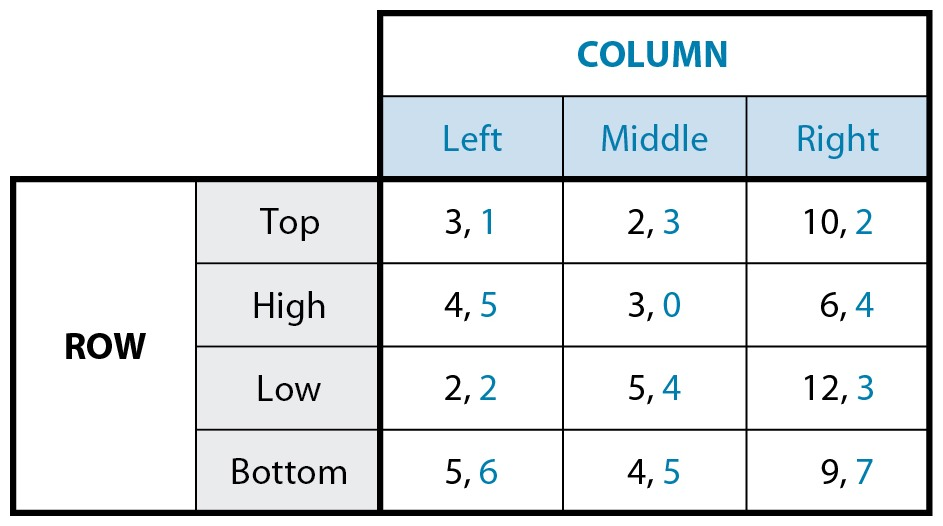
\includegraphics[width=.75\textwidth]{./img/GAMES4_FIG04.01.jpg}
\end{center}
\end{frame}

\begin{frame}[label={sec:orga65aae8}]{}
\alert{Example: American football play}
\begin{itemize}
\item Offensive team chooses from among types of plays
\item Defensive team simultaneously chooses type of play to counter offense
\item Payoffs are zero-sum: whatever offense gains (in yards) is equal to what the defense loses
\end{itemize}
\end{frame}

\begin{frame}[label={sec:orgaaaef25}]{}
\begin{center}
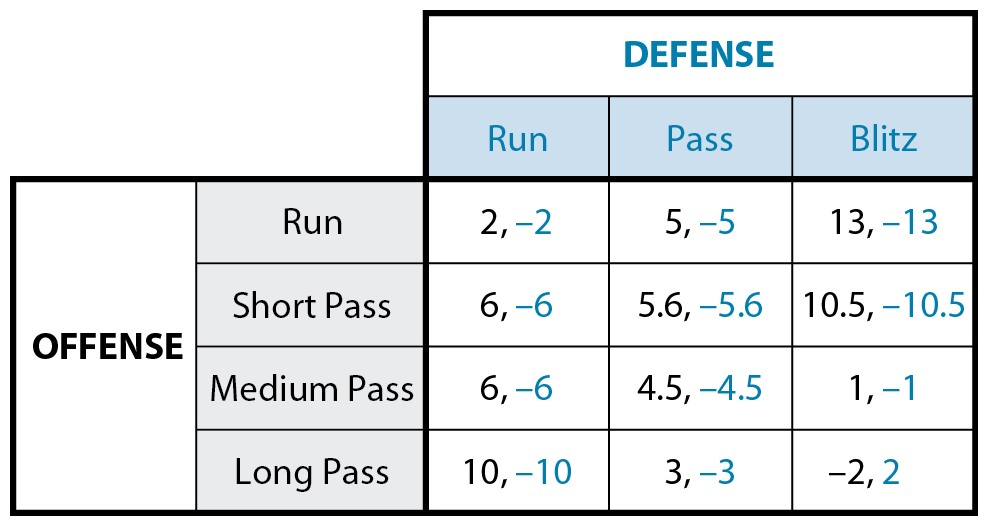
\includegraphics[width=.75\textwidth]{./img/GAMES4_FIG04.02.jpg}
\end{center}
\end{frame}

\begin{frame}[label={sec:orge548e35}]{Example: Pricing game}
\end{frame}

\begin{frame}[label={sec:org92d2af1}]{}
\alert{Best response}
\begin{itemize}
\item We can analyze simultaneous move games by describing player's \emph{best response} actions
\item The best response is the action that maximizes a player's payoffs \emph{given} the action of the opposing player(s)
\item \emph{If} the other player does X, \emph{then} I should do Y
\end{itemize}
\end{frame}

\begin{frame}[label={sec:org024ba13}]{Suppose Row plays top:}
\begin{center}
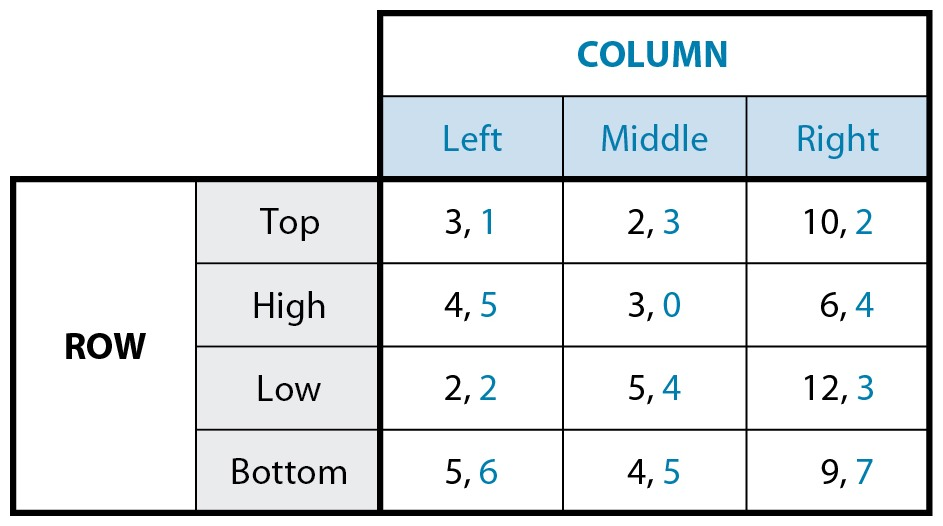
\includegraphics[width=.75\textwidth]{./img/GAMES4_FIG04.01.jpg}
\end{center}
\end{frame}

\begin{frame}[label={sec:org83a0cbb}]{}
\alert{Nash equilibrium}
\begin{itemize}
\item Nash equilibrium occurs when both players are \emph{simultaneously} choosing their best-response actions
\item Neither player can achieve higher payoffs by changing their actions \emph{given} the action of the other player
\item Not necessarily the best outcome for both players
\end{itemize}
\end{frame}

\begin{frame}[label={sec:org31188d4}]{Nash equilibrium: (Low, Middle)}
\begin{center}
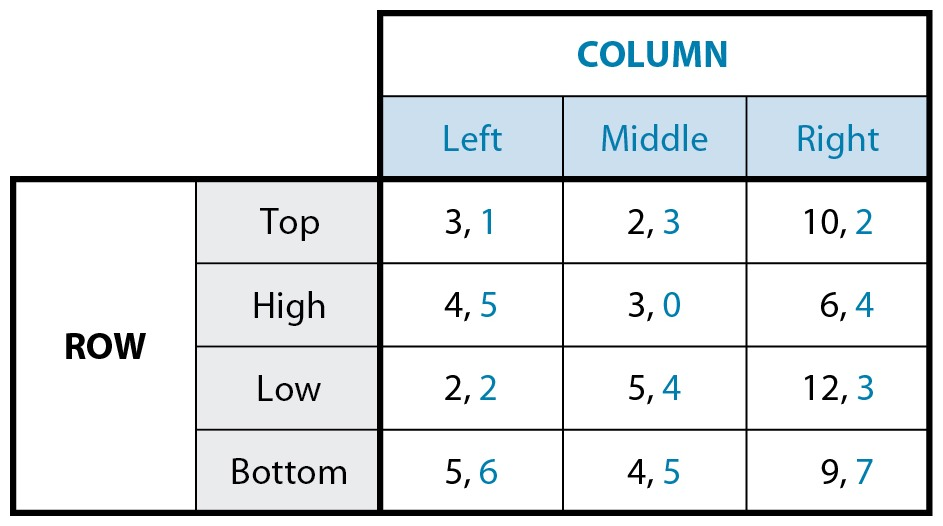
\includegraphics[width=.75\textwidth]{./img/GAMES4_FIG04.01.jpg}
\end{center}
\end{frame}

\begin{frame}[label={sec:org2761500}]{Still a Nash equilibrium?}
\begin{center}
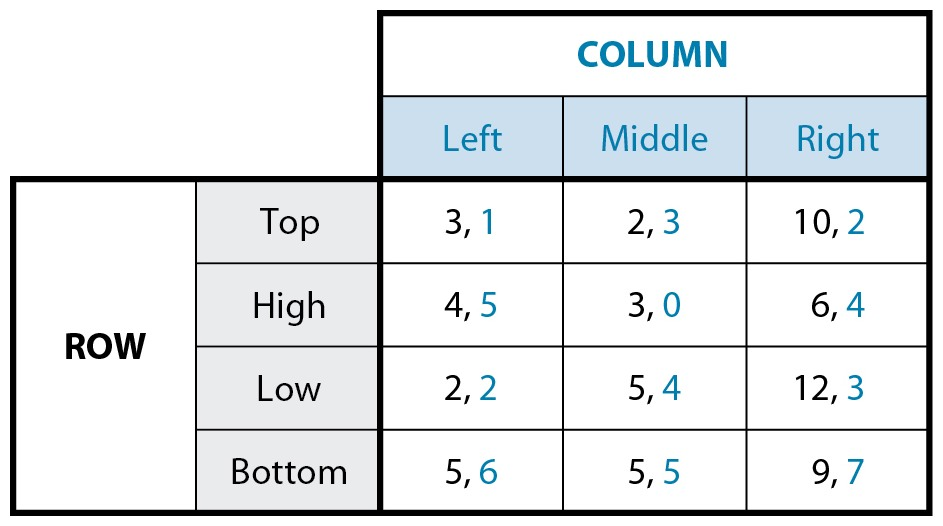
\includegraphics[width=.75\textwidth]{./img/GAMES4_FIG04.03.jpg}
\end{center}
\end{frame}

\begin{frame}[label={sec:orgc1c5e8a}]{}
\alert{Beliefs}
\begin{itemize}
\item How can a player choose a best "response" if they are playing simultaneously?
\begin{itemize}
\item What are they responding to?
\end{itemize}
\item Players form \emph{beliefs} about what other players will do
\item At the Nash equilibrium:
\begin{itemize}
\item All players choose optimal actions given their beliefs about what other players are doing
\item The beliefs are accurate
\end{itemize}
\item If either condition doesn't hold, then not a Nash equilibrium
\end{itemize}
\end{frame}

\begin{frame}[label={sec:org3619743}]{Will Row play Low if they believe Column isn't playing Middle?}
\begin{center}
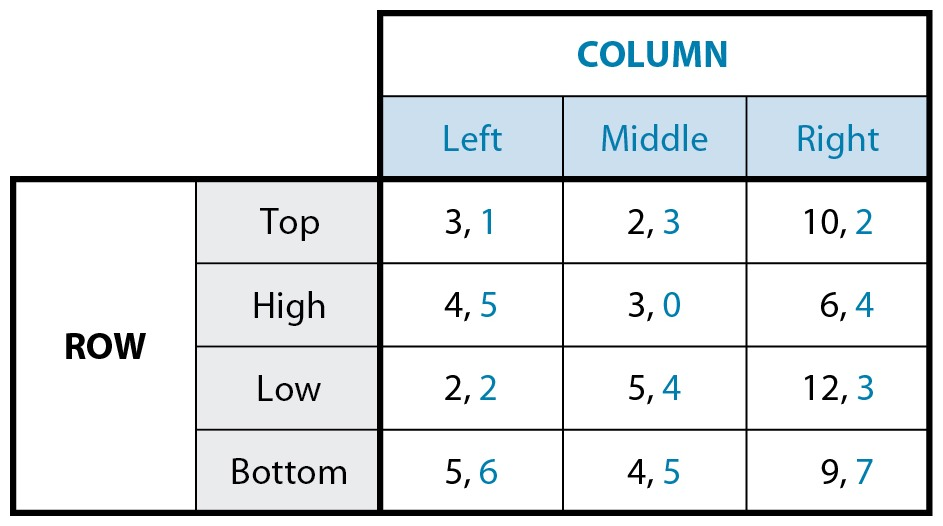
\includegraphics[width=.75\textwidth]{./img/GAMES4_FIG04.01.jpg}
\end{center}
\end{frame}


\begin{frame}[label={sec:orgeb34651}]{What is the Nash equilibrium?}
\begin{center}
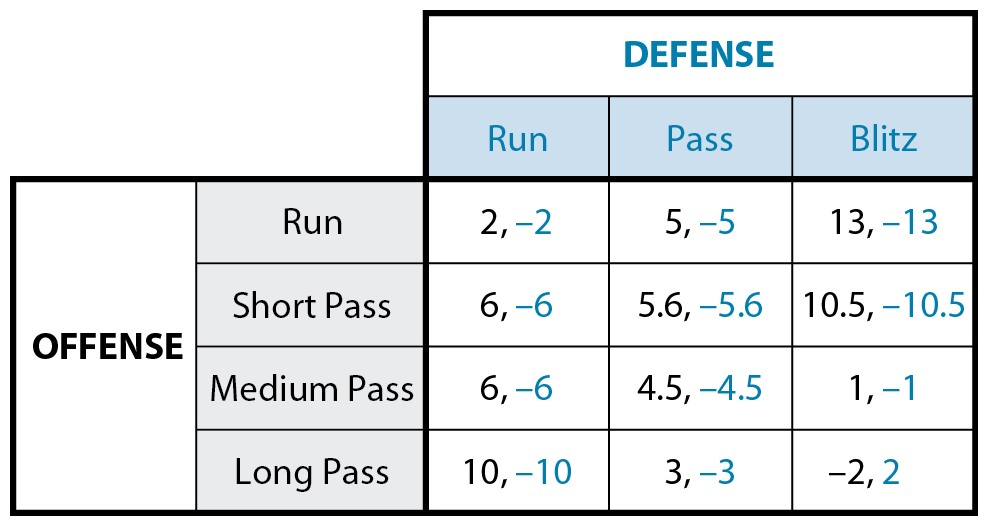
\includegraphics[width=.75\textwidth]{./img/GAMES4_FIG04.02.jpg}
\end{center}
\end{frame}

\begin{frame}[label={sec:orgc12bf41}]{}
\alert{Extra credit}
\begin{itemize}
\item Write your name at the top of a blank sheet of paper
\item Answer the following questions. For each answer that is the same for \emph{everyone else}, you will receive 2 points extra credit on the homework
\begin{enumerate}
\item Select "Heads" or "Tails"
\item Choose one of the numbers 7, 100, 13, 261, 99, 555
\item You are to meet someone in Corvallis. You have not been instructed where to meet, you have no prior understanding with the person on where to meet, and you cannot communicate with each other. You are simply told that you will have to guess where to meet, that the other person is being told the same thing, and that you will just have to try to make your guesses coincide. Where do you go?
\item You are told the date but not the hour of the meeting in question 3. The two of you must guess the exact minute of the day for the meeting. At what time will you appear?
\item Write some positive number.
\end{enumerate}
\end{itemize}
\end{frame}
\end{document}